
\chapter{Transport calculations}
\label{app:transp}

Non-equilibrium Green's function calculations are now possible with
{\dftbp}. Within this formalism it is possible to treat quantum mechanical
systems with open boundary conditions and therefore quantum transport.  A
specific new \kwcb{Transport} block has been added to control the transport
problem.  The NEGF solver parameters can be controlled within the
\kw{Eigensolver} section, using the keyword \kwcb{GreensFunction}. Finally the
real-space Poisson solver parameters have been organized within a new section,
\kw{Electrostatics}, using the keyword \kwcb{Poisson}. The default value for the
electrostatic calculations is the usual $\gamma$-functional which contains the
Hartree and local XC potential.

\section{Definition of the geometry}

The input geometry for transport calculations is a little tricky. In comparison
to cluster or supercell calculations the geometry for transport calculation must
also contain information about the contacts. The contacting leads are actually
semi-infinite structures, supporting travelling waves. No stationary current is
possible in a finite structure, as travelling waves can only exist in open
systems.  The structure is partitioned into a device region and two or more
contact regions.

Rules to build a valid input structure:
\begin{enumerate}
\item \label{rule1} All device atoms must come first.
\item \label{rule2} Each contact must comprise two subsequent unit cells called
  principal layers (PLs). The two PLs together give all information about the
  contact structure and in the following are referred generally as 'contact'.
\item \label{rule3} A PL is a unit cell of the contacting lead that has
  interactions only with nearest neighbour PLs in tight-binding terms.
\item \label{rule4} The ordering of the atoms within the two PLs must be
  consitent in the sense that the two PLs must be exact periodic replica of each
  other: If each PL comprise N atoms, atom M in the first PL must have a
  corresponding identical atom in the second PL at position M+N.
\item \label{rule5} The first PL should be always the one closer to the device
  region.
\item \label{rule6} All blocks should be contiguous in the structure and each
  atom must belong to one and only one region.
\item \label{rule7} The geometry can be defined as a cluster or a supercell. In
  the first case is it understood that the contacts are just one-dimensional
  wire leads.
\item \label{rule8} If a structure is defined as {\em supercell}, only the
  lattice vectors transverse to the transport direction are meaningful. The
  periodicity specified along the transport direction is dummy.
\item \label{rule9} For each contact the periodicity along the transport
  direction is deduced from the separation between the two PLs (as the
  coordinate difference $\mathbf{r}(M+N)-\mathbf{r}(M)$). We refer to this as
  {\em contact direction}.
\item \label{rule10} All lattice vectors (including the periodicity vector of
  the contacts) must be aligned to one of the cartesian axes x, y or z. In
  practice only rectangular cells are currently allowed in transport
  calculations.
\end{enumerate}
 
Note: Currently the code makes only a consistency check on the definition of the
two PLs (rule~\ref{rule4}), namely it checks whether the two contact PLs are
really shifted copies of each other.  The code does not check if the device
regions are consistently defined (rules~\ref{rule1} and \ref{rule6}), if the PL
defined are really PLs (rule~\ref{rule3}) and does not check if the first PL
defined is really the one closest to the device (rule~\ref{rule5}).  The code
checks rules \ref{rule8}, \ref{rule9} and \ref{rule10}. The check is performed
    on the atomic coordinates, such that
\begin{equation} 
 \mathbf{R}^2_{i+N} = \mathbf{R}^1_i + \mathbf{v}\qquad\forall i \in PL 
\end{equation}
where $\mathbf{R}^2_i$ are atomic coordinates of atoms in the second PL,
$\mathbf{R}^1_i$ are atomic coordinates of atoms in the first PL and
$\mathbf{v}$ is the contact lattice vector. The equality is verified within an
accuracy that can be set by the user (see below).

Please take your time to build up structures and cross-check them. Also consider
to look at the examples distributed with the code. The input structure is often
the first suspect when there's some problem in the calculation.

    
\htsection{Transport} 

\dftbp{} allows for NEGF calculations on different levels. It is possible to
calculate linear response transmission within Landauer formalism, charge density
out of equilibrium with self-consistent schemes, local currents etc. The
Transport section groups the information needed whenever open boundary
conditions are used. It contains the description of the partitioning of the
system into {\em device} and {\em contact} regions and additional contact
information needed to calculate the associated Self Energies. The transport
block contains the following properties:

\begin{ptable}
  \kw{Device} &p& & - & \pref{Device} \\
  \kw{Contact} &p& & - & \pref{Contact} \\
  \kw{Task} & m & & UploadContacts & \pref{Task} \\
  \hline
\end{ptable}


Example: 

\begin{verbatim}
Transport {
    Device {
      AtomRange = 1 8 
    }
    Contact {
      Id = "source"
      AtomRange = 9 24 
    }
    Contact {
      Id = "drain"
      AtomRange = 25 40
    }
  Task = ContactHamiltonian
}
\end{verbatim}


\htcbsubsection{Device} The Device blocks contains the following properties:

\begin{ptable}
  \kw{AtomRange} &2i& & - & \pref{AtomRange} \\
  \kw{FirstLayerAtoms} &i+& & 1 &  \\
  \hline
\end{ptable}

\begin{description}

\item[\is{AtomRange}] defines the first and last atom of the device region.

\item[\is{FirstLayerAtoms}] defines the first atom of PLs in the device
  region. By default there is only one layer (the entire device
  region). Alternatively the user can manually reorder and partition the
  structure into layers for efficient GF calculations.
  
  Differently from the contact PLs, the device layers do not need to represent
  unit cell repetitions. The device geometry must be manually ordered in such a
  way that all the atoms within each layer are contiguous and adjacent layers
  are placed next to each other. This ensures that the constructed Hamiltonian
  and Overlap are block tri-diagonal. Refer to \cite{Pecchia_NJP} for a
  description of the iterative algorithm.

\end{description}
 
\htcbsubsection{Contact} The contact block contains the following properties:

\begin{ptable}
  \kw{Id} & s &  & &  \\
  \kw{AtomRange} &2i& &  &  \\
  \kw{ShiftAccuracy} & r & & 1e-8 & \\
  \kw{FermiLevel} &r& &  &  \\
  \kw{Potential} & r &  & 0.0 & \\
  \kw{WideBand} & l & & No & \\
  \kw{LevelSpacing} & r & WideBand = Yes & 20.0 & \\
  \hline
\end{ptable}

The sections \verb|Device| and \verb|Contact| are used to define the atomic
range of each region. The user can also assign a label (\is{Id}) to each contact
that can be used later for cross referencing. In the section \verb|Contact| the
user can add a keyword that specifies the accuracy for the internal check of the
PLs.

\begin{description}
\item[\is{Id}] Assign a label to each contact. 
\item[\is{AtomRange}] \label{AtomRange} Defines the first and last atom of the
  device region.  {\bf Note} that the contacts should be defined in order of
  increasing atomic range.

\item[\is{ShiftAccuracy}]\modif{\modtype{length}} It can be used to set the
  absolute accuracy used to check the PL consistency (see above). The default is
  $10^{-5}$ atomic units. Please be aware that using a large values may hide
  errors due to a non consistent definition of the contacts, therefore it should
  not be modified.
  \item[\is{FermiLevel}]\modif{\modtype{energy}} Specifies the contact Fermi
    levels.
  \item[\is{Potential}]\modif{\modtype{energy}} Specifies the electrostatic
    potential applied to each contact. The natural units of this quantity are
    potential energy (e.g., V). They can be loosely identified with eV or
    a.u. since in both these units the electronic charge is practically defined
    as $e=1$.
  \item[\is{WideBand}] Use the wide band approximation for the contact. If set
    to Yes, the surface green's function of the contact is not explicitly
    calculated but rather assumed to be local and constant according to a
    specified density of states.
  \item[\is{LevelSpacing}]\modif{\modtype{energy}} Specify the inverse of the
    density of states per atom to be used in the Wide Band approximation. As an
    example, the DOS of gold at the Fermi level is $0.05
    \mathrm{ev}^{-1}\mathrm{atom}^{-1}$, which corresponds to an energy spacing
    of $20$ Ev $ \simeq 0.735$ Hartree (the default value).
\end{description}

\htcbsubsection{Task = ContactHamiltonian} \label{Task} The \is{Task} option is
used to define which type of calculation should be performed. Before an SCC
transport calculation it is necessary to compute some equilibrium properties of
the contacts, by running a periodic boundary conditions DFTB calculation.This
necessary step must be carried separatley for each contact and can be done by
specifying setting \kw{Task}=\is{ContactHamiltonian} as in the following example

\begin{verbatim}
Task = ContactHamiltonian {
  ContactId = source
  ContactSeparation [Angstrom] = 50.0 
}
\end{verbatim}

When \kw{Task}=\is{ContactHamiltonian} the following options can be defined

\begin{ptable}
  \kw{ContactId} & s &  & &  \\
  \kw{ContactSeparation} & r & & 1e3 &  \\
  \hline
\end{ptable}

\begin{description}
\item[\is{ContactId}] Id of the contact to be calculated.
\item[\is{ContactSeparation}]\modif{\modtype{length}} Dummy separation in
  transverse direction (see following explanation).
\end{description}

The contact calculation computes the {\em bulk} Hamiltonian and self-consistent
charges for each contact. This is a usual \dftbp calculation for which
appropriate parameters must be included in the input file. For {\em supercell}
structures the calculation of the contact is performed using corresponding
supercells in which the transverse lattice vectors are those specified in the
\is{Geometry} tag and the lattice vector along the {\em contact direction} is
deduced from the PL separation (rule~\ref{rule9}). If the structure is defined
as a {\em cluster}, the contact calculation is performed for a {\em supercell}
in which the contact is treated as one-dimensional wire. However, since \dftbp
does not support pure one- and two-dimensional calculations, dummy lattice
vectors are defined for the two remaining directions. The default value for
these lattice vectors is 1000 a.u. (527 \AA), which should guarantee sufficient
wire-wire distance to avoid Coulomb interactions. The user can specify and
alternative contact separation using the keyword \is{ContactSeparation} placed
in the \kw{ContactHamiltonian} block.  Each contact computation produces one
output file called \verb|shiftcont_ContactId.dat| storing energy shifts and
Mulliken charges that must be present in the working folder in all subsequent
transport calculations.

{\bf Note} that during the contact calculation you will need to perform a
k-point integration.  Whenever the system is defined as a cluster, \dftbp{} will
authomatically extract the periodicity vectors from the geometry such that the
first reciprocal vector will correspond to the contact direction.  Therefore you
must specify the k-point sampling for the periodic calculation by sampling along
the first reciprocal lattice vector.  As an example, if the structure is defined
as a cluster (i.e., 1-dimensional wire leads), the source contact calculation
will have an input file similar to:

\begin{verbatim}
...
Task = ContactHamiltonian {
  ContactId = source
}
...
Hamiltonian = DFTB {
...
KpointsAndWeights = SupercellFolding {
     8  0  0   # Regardless of transport direction
     0  1  0
     0  0  1
     0.5 0.0 0.0
  }

}
\end{verbatim}

On the other hand, if your structure is defined as a supercell (as an example, a
molecule with bulk contacts) and the transport direction is along y, your the
source contact calculation will have an input file similar to:

\begin{verbatim}
...
Task = ContactHamiltonian {
  ContactId = source
}
...
Hamiltonian = DFTB {
...
KpointsAndWeights = SupercellFolding {
     4  0  0   # Folding in parallel direction
     0  8  0   # Folding in transport direction
     0  0  4   # Folding in parallel direction
     0.5 0.5 0.5
  }

}
\end{verbatim}


This could seem confusing, but the underlining reasons is that in the cluster
calculation the reciprocal lattice is set up by the code itself, while in the
periodic calculation is set up by the user who can chose any arbitrary
direction.  Refer to the transport cookbook and to the distributed examples for
further clarification.

\htcbsubsection{Task = UploadContacts} After the contact calculations, it is
possible to perform actual transport calculations. This is activated simply
specifying \kw{Task = UploadContacts}, without additional options. In order to
set a proper transport calculation the user should also define the FermiLevel
and Potential to each contact.
\begin{verbatim}
Transport {
  Device {
    AtomRange = 1 8
  }
  Contact {
    Id = "source"
    AtomRange = 9 24
    FermiLevel [eV] = -8.4123
    Potential = 0.0 
  }
  Contact {
    Id = "drain"
    AtomRange = 25 40
    FermiLevel [eV] = -8.4123
    Potential = 1.0 
  }
  Task = UploadContacts
}
\end{verbatim}

Note: During the transport calculation you will not need to set up the k-point
integration when the structure is defined as a cluster, just as in a regular
\dftbp{} calculation.

 
\htsection{GreensFunction} 

In order to activate Green's functions calculations the user must define the
keyword \is{EigenSolver = GreensFunction} in the \is{Hamiltonian} section. The
Green's function section describes all the parameters needed by the Green's
function (GF) solver. The GF solver, either under equilibrium (no bias applied)
or under non-equilibrium conditions, builds up the density-matrix of the device
region. Strictly speaking the GF does not solve for the eigenstates of the open
system, however it logically substitutes the traditional construction of the
density matrix from the eigenstates of the system, obtained after the
diagonalization step. The density matrix can be used to compute any physical
observable by 'tracing' with the appropriate operator. In particular it is
possible to calculate the Mulliken charges necessary for the DFTB
self-consistent loop. Therefore the usual \dftbp ~self-consistent calculations
can be driven using the GF solver. The Green's function section contains
important parameters used by the solver. The following table describes these
parameters.

\begin{ptableh}
  \kw{Delta} & r  &  & 1e-5 & \\
  \kw{ContourPoints} & 2i &  & 20 20 &  \\
  \kw{LowestEnergy}  & r  &  & -2.0 & \\
  \kw{FermiCutoff}  & i & & 10 & \\
  \kw{EnclosedPoles} & i & & 3 & \\
  \kw{RealAxisStep} & r & RealAxisPoints=undefined & 6.65e-4 & \\
  \kw{RealAxisPoints} & r & RealAxisStep=undefined &  & \\
  \kw{SaveSurfaceGFs} & l & & Yes & \\
  \kw{ReadSurfaceGFs} & l & & No & \\
  \kw{FirstLayerAtoms} & i+ & Transport = undefined & 1 & \\
  \kw{FermiLevel} & r& Transport = undefined &  & \\
  \kw{LocalCurrents} & l&  & No & \\
\end{ptableh}

Note: For efficient GF calculation the device region must be partitioned into
layers whose fundamental property is to interact with nearest-neighbour layers
only.

\begin{description}
\item[\is{Delta}]\modif{\modtype{energy}}\modif{\modtype{energy}} A small
  positive imaginary delta used in the GF definition.
  \item[\is{ContourPoints}] The number of points along the complex contour
    integration of the GF along the contour segments $\mathcal{C}$ and
    $\mathcal{L}$ (see contour integration).
\item[\is{LowestEnergy}]\modif{\modtype{energy}}\modif{\modtype{energy}} The
  initial energy from which the integration starts. It should be low enough to
  ensure that all the electronic states are correctly included in the
  integration. The default is -2.0 Hartree (see contour integration).
\item[\is{FermiCutoff}] Integer number setting the Fermi distribution cutoff in
  units of $kT$. It is read only if the Fermi distribution temperature is
  greater than 0 (see contour integration).
\item[\is{EnclosedPoles}] The number of Poles enclosed in the contour. It is
  meaningful only in finite temperature calculations (see contour integration).
\item[\is{RealAxisStep}]\modif{\modtype{energy}} The energy step along the real
  axis integration for non-equilibrium calculations. Note: \kw{RealAxisStep} and
  \kw{RealAxisPoints} can not be both defined at the same time.
 
  \item[\is{RealAxisPoints}] The number of points along the real axis
    integration needed in non-equilibrium calculations. The default depends on
    the electronic temperature and bias. Note: \kw{RealAxisStep} and
    \kw{RealAxisPoints} can not be both defined at the same time.
 
\item[\is{SaveSurfaceGFs}] As the SCC cycle usually needs to repeat the
  calculation of the Green's function at given energy points and as the surface
  Green functions do not change during the SCC cycle, this flag allows for
  saving the surface Green functions to disk and save computational time on
  every SCC cycle beyond the first.

\item[\is{ReadSurfaceGFs}] Allow to load surface Green's function from file also
  at the first SCC cycle. Note that this operation only makes sense if the
  energy integration points are identical to the calculation used to generate
  the surface Green's function files. The code do not verify whether this
  condition s fulfilled. In general there is no need to modify this default for
  \kw{ReadSurfaceGS} and \kw{SaveSurfaceGS}.

Note: the Green solver can be used also to calculate the density matrix when
there is no open buondary conditions, for example to take advantage of the
iterative scheme in quasi-1d systems. In this case, a \kw{Transport} block is
not defined and therefore \iscb{FirstlayerAtoms} should be defined here. Also, a
Fermi level of the system must be known and provided to fill up the electronic
states.
      
\item[\is{FirstLayerAtoms}] As described in Device block. Can be specified only
  if no \kw{Transport} block exists.

\item[\is{FermiLevel}]\modif{\modtype{energy}} The Fermi level used by the Green
  solver to fill up the electronic states.

\item[\is{LocalCurrents}] if set to Yes, local bond-currents are computed using
  the non-equilibrium density matrix.  This task is currently limited to
  non-periodic systems. The output is placed in a file \verb|lcurrent_u.dat| (or
  \verb|lcurrent_d.dat| dending on spin).  The files are arranged in a table in
  order of increasing neighbour distance,

\begin{tabular}{|c|c|c|c|c|c|c|c|c|c|c|c|}
  \hline
  Atom(i) & x & y & z &  nNeighbors &  j1 & I$_{i,j1}$ & j2 & I$_{i,j2}$ &  j3 & I$_{i,j3}$ & ...\\ 
  \hline
\end{tabular}

  This file can be processed using the small code \verb|flux| provided in
  tools/transport that helps in building plots for jmol.
\end{description}

GreensFunction section example:

\begin{verbatim}  
Eigensolver = GreensFunction {
  FirstLayerAtoms = 1 61 92 145
  Delta [eV] = 1e-4
  ContourPoints = 20 20
  RealAxisPoints = 55
  LowestEnergy [eV] = -60.0
  FermiCutoff = 10
  EnclosedPoles = 3
}
\end{verbatim}


  Note: in order to solve the self-consistent NEGF transport problem, the
  GreensFunction Eigensolver must be used. However, the \iscb{TunelingAndDos}
  section can be used to calculate the transmission coefficients according to
  Landauer formula in a non self-consistent manner. In this case an Eigensolver
  is not needed as the charge density doesn't need to be calculated.  To run
  such a calculation, \is{Eigensolver = TransportOnly} must be set and no
  electrostatics must be calculated (i.e. the \is{Electrostatics = Poisson}
  should not be declared).


\section{Contour integration}

Much of the computational work is in the integration of the energy resolved
density matrix, represented via the NEGF matrix. The integration is efficiently
performed with a complex contour integration and a real axis integration, as
shown in Figure~\ref{fig:contour} and discussed in references \cite{Pecchia_RPP,
  Pecchia_spring, Pecchia_NJP}.
\begin{figure}[!h]
\begin{center}
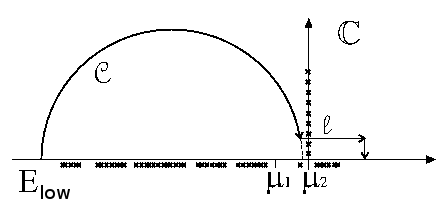
\includegraphics[width=8.0cm]{Fig_integration.png}
\caption{ \label{fig:contour} Contour integration in the complex plane for the
  Green's fuctions. The crosses represent poles of either $G^r$ or the Fermi
  function.}
\end{center}
\end{figure}
All integrations are performed with Gaussian quadratures and the number of
points must be specified manually. The complex contour integration is subdivided
into two sections: the first section is an arc of circle, $\mathcal{C}$, that
can be computed with few integration points (default 20); the second section is
a line that intersects the contour and runs parallel to the real axis at a
distance that depends on the number of poles of the Fermi function enclosed
within the contour. Usually a good choice for the number of poles is between 3
and 5 (the default is 3). The poles are placed at the complex points $z_m = E_F
+ i (2m+1) \pi k T$ and, therefore, are separated from each other by $2 \pi k
T$.  At $T=300$~K this corresponds to a separation of 156~meV. It should be
noted that, as the temperature decreases, the separation between poles
reduces. This makes the contour integration harder as it needs to walk across
two singularities. At very low temperatures, $T=10$~K, the separation is 5.2
meV. Below this temperature the contour integration is treated as $T=0$ in order
to avoid numerical inaccuracies. The integration along the segment $\mathcal{L}$
extends up to $Re\left[ z \right]=E_F+nkT$, where $n$ is an integer number
specified by the keyword \kw{FermiCutoff} and has a default value of 10.  In the
limit $T=0$~K the poles collapse into a non-analytic cut and the contour needs
to be changed such that the second section of the complex contour becomes the
arc of circle closing on the real axis.  Finally, the real axis integration
extends between the lowest and highest chemical potentials. The number of
quadrature points should depend on the bias itself and can be set using
\kw{RealAxisPoints} or \kw{RealAxisStep}. The default value is
$1\text{~pt}/0.018\text{~eV}$ (actually $1500\text{~pt}/1\text{~H}$). In finite
temperature calculations the segment is extended to include the Fermi cutoff by
$nkT$ on both sides ($\mu_1-nkT, \mu_2+nkT$). In this case the number of
quadrature points are increased by assuming the same point density defined in
the range ($\mu_1, \mu_2$).  Example: for a bias of 0.2 V, the default number of
points is $0.2\cdot1500/27.21139=11$. At $T=300$~K the interval is increased by
0.26~eV on both sides, therefore $0.26\cdot1500/27.21139=14.33$ which is
truncated to 14 points, leading to a total of 38 points along the real axis. The
use of the keyword \kw{RealAxisStep} is usually more convenient because it
ensures a consistent real axis integrations during, for example, a bias sweep.

Note: The GF solver can be used also for calculations other than the transport
context. In case the position of the Fermi Energy is known with good accuracy
the density matrix solver based on the GF can be used to compute the electronic
properties of clusters and supercells. The recursive algorithm may be an
efficient solution to large problem and could be efficient for systems having an
elongated 1D shape.

\section{Poisson solver}

The Poisson solver is a fundamental part of the non-equilibrium transport
calculations and must be declared whenever a NEGF calculation is performed using
\is{Electrostatics = Poisson}. Under non-equilibrium conditions the
self-consitent potential of the KS equations cannot be solved using the
efficient $\gamma$-functional, but requires the definition of appropiate
boundary conditions for the potentials imposed on the contacts. However, since
the $\gamma$-functional is formally identical to a pure Hartree potential, it
can be obtained in real space by solving a Poisson solver.  The Poisson equation
is solved in a {\em box} with hexahedral prism shape. This restriction is
imposed by the solver employed. This restricts calculations of supercell
structures to orthorhombic super-lattices.  An additional restriction is that
the box sides must be aligned with the Cartesian axes, x, y, z.

\begin{ptableh}
  \kw{PoissonBox} & 3r & &  &  \\
  \kw{MinimalGrid} & 3r  &  & 0.5 0.5 0.5 & \\
  \kw{PoissonAccuracy} & r &  & 1e-7 &  \\
  \kw{AtomDensityTolerance}  & r  &  & 1e-6 & \\
  \kw{CutoffCheck} & l & & Yes & \\
  \kw{Verbosity} & i & & 51 & \\
  \kw{SavePotential} & l & & No & \\
  \kw{PoissonAccuracy} & r & & 1e-6 & \\
  \kw{MaxPoissonIterations} & i & & 60 & \\
  \kw{BuildBulkPotential} & l & & Yes & \pref{Boundary Conditions}\\
  \kw{ReadOldBulkPotential} & l & & Yes & \pref{Boundary Conditions} \\
  \kw{OverrideDefaultBC} & m & & none\{\} & \pref{Boundary Conditions}\\
  \kw{OverrideBulkBC} & m & & none\{\} & \pref{Boundary Conditions}\\ 
  \kw{BoundaryRegion} & m & & global\{\} &  \pref{Boundary Conditions} \\
  \kw{Gate} & m & & none\{\} & \pref{Electrostatic Gates} \\ 
  \kw{MaxParallelNodes} & m & & none\{\} & \pref{Parallelizations} \\ 
\end{ptableh}



\begin{description}
\item[\is{PoissonBox}]\modif{\modtype{length}} Dimension of the Poisson box
  along directions x, y and z.
\item[\is{MinimalGrid}]\modif{\modtype{length}} The minimal requested grid
  spacing along x, y and z. The actual grid spacing chosen by the multigrid will
  be lower than this.  charge densities.
  \item[\is{AtomDensityTolerance}] In order to calculate the potential, the
    Mulliken charges are projected on the real space grid. This parameter
    defines the cutoff after which the charge is considered vanish (i.e., the
    space extension of the projected charge). The default is 1e-6. Note that the
    contacts must be at least twice the length of the extent of a projected
    Mulliken charge. If this conditions is not fullfilled and is set to Yes, the
    code will exit with an error message. Setting this parameter to a lower
    value could allow to define shorter contacts in some cases. However this
    could lead to relevant error in the potential hence to spurious reflections,
    therefore it should be left to default value or changed very carefully.
  \item[\is{CutoffCheck}] If set to No, consistency between contact length and
    charge extension is not verified (see above section). The default is No. As
    for AtomDensityTolerance, this parameter shouldn't be touched unless you
    know exactly what you're doing.
  \item[\is{Verbosity}] This parameter controls the amount of output messages
    and takes values ranging from 1 to 100.
  \item[\is{SavePotential}] Save the potential to file. 
\item[\is{PoissonAccuracy}] Defines the accuracy for the approximate solution of
  the Poisson equation (default value 10$^{-6}$).
\item[\is{MaxPoissonIterations}] Defines the maximum amounts of iterations for
  the solver.
\end{description}

{\bf Note}: The Poisson Box can be specified using the keyword
\verb|PoissonBox|. In calculations in which the two contacts face each other
along the same axis, setting the box-size along this axis has no effect because
the code needs to adjust the correct size internally.  This keyword is redundant
(and should not be specified) when the system is periodic, since in this case
the Poisson box is taken from the supercell lattice vectors.

Numerical error in the potential will results in spurious discontinuities at the
contact-device interfaces. The default tolerances should do the job in most
cases.

This is a tipical example of the whole Poisson block specification. Some of the
keywords are described in the next subsections.


Example:
 
\begin{verbatim}
 Electrostatics = Poisson {
  PoissonBox [Angstrom] = 20.0 20.0 20.0
  MinimalGrid [Angstrom] = 0.3 0.3 0.3
  SavePotential = No
  BuildBulkPotential = Yes
  ReadOldBulkPotential = No
  BoundaryRegion = Global {}
  PoissonAccuracy = 1e-7
  Gate = Planar{
      GateLength_l [Angstrom] = 10.0
      GateLength_t [Angstrom] = 20.0
      GateDistance [Angstrom] = 7.0
      GatePotential [eV] = 1.0
  }
}
\end{verbatim}

\htsubsection{Boundary Conditions}

The Poisson equation is solved imposing special boundary conditions (BC) on the
six faces of the Poisson Box. In basic transport calculations, comprising two
contacts placed along the same axis, the BCs are choosen as follows:

\begin{description}
\item[Dirichlet] Fixed potentials on the two contact faces with values defined
  by the applied potentials (see \is{UploadContacts}, \is{ContactPotentials}).
\item[Neumann] Zero normal field on the remaining 4 lateral box faces.
\end{description}
In periodic supercells the BCs are: {\bf Dirichlet} (fixed potentials) on the
two contact faces with values defined by the applied potentials (see
\is{UploadContacts}, \is{ContactPotentials}) and {\bf Periodic} on the remaining
4 lateral box faces.

In some specific cases Neumann BCs can be set on one contact. In order to do so
it is necessary to use \verb|OverrideDefaultBC| (see below).

Device and contact potentials should smoothy join at the interface. In order to
reach this goal the code computes the Bulk potential of each contact and uses
the result as a BC on the contact face of the Poisson box. This is useful when
the contact potential is not uniform due to charge rearrangments. The external
applied contact potential is added to the bulk potential.  The user can
deactivate this calculation with the keyword \kw{BuildBulkPotential}.

{\bf Note}: The bulk potential is computed on a special box that has 'lateral'
sizes copied from the device box, and has the size of one PL along the contact
direction. The BCs are --so to speak-- inherited from the device region. In
particular:
\begin{enumerate}
\item Along the contact direction periodic BCs are imposed.
\item On the other four faces the BCs are copied from the device region.
\item The user can override this setting using \verb|OverrideBulkBC| (see
  below).
\item When all four faces inherit Neumann BC (default for the device region),
  these are ALL internally changed to Dirichlet, because the solver cannot
  handle this situation that gives rise to a singular matrix.
\end{enumerate}

\begin{description}
\item[\is{BuildBulkPotential}] (default: \is{Yes}) is used to calculate the
  electrostatic potential of the contacts and the result is used as a Dirichlet
  boundary condition on the contact face (superimposed to the contact
  potential).
\item[\is{ReadOldBulkPotential}] Read a previously computed bulk potential from
  hard-disk.
\item[\is{BoundaryRegion}] Specifies how the Dirichlet boundary conditions are
  treated on each contact face of the Poisson box. It can be \kw{Global},
  \kw{Square} or \kw{Circle}. \kw{Global} means that the BC is applied to the
  entire face of the box, whereas the other keywords imply that the Dirichlet
  BC are applied on a cross-section projected on the contact face. This is
  useful for instance when handling nanowire contacts, for which it is not
  really consistent to impose a constant potential on the whole face of the
  Poisson box.
\item[\is{BufferLength}]\modif{\modtype{length}} can be used to set the size of
  the boundary region beyond the atomistic size which is determined as the
  minimal circle or qquare containg all atoms of the contact cross-section.
\end{description}

Example:
\begin{verbatim} 
BoundaryRegion = Circle {
    BufferLength [Angstrom] = 3.0 
}  
\end{verbatim}

In some special case it might be necessary to override the default BCs applied
by the code on the Poisson equation. Currently this can be done using the
keywords: \verb|OverrideDefaultBC| and \verb|OverrideBulkBC|.

\begin{description}
\item[\is{OverrideDefaultBC}] block is used to override the BCs described
  above. It can be used to force Dirichlet or Neumann BCs along some specified
  directions or on one of the four lateral faces of the Poisson box.
\item[\is{Boundaries}] is used to specify on which face different BCs must be
  imposed. Assuming contacts along z, the keyword can be set any of xmin, xmax,
  x, ymin, ymax, y.
\end{description}

\begin{verbatim}
OverrideDefaultBC = Dirichlet {
      Boundaries = xmin   
}
\end{verbatim}

For instance setting Dirichlet BC on \verb|Boundaries = xmin| imposes
$\phi(x,y,z)=0$ on the face placed at $x=x_{\text{min}}$,
\verb|boundaries = xmax| imposes $\phi(x,y,z)=0$ on the face placed at
$x=x_{\text{max}}$. When Dirichlet needs to be forced on both faces, it is
possible to use either \verb|boundaries = xmin,xmax| or simply
\verb|boundaries = x|. The same syntax can be used to impose conditions on more
faces, using \verb|boundaries = x,y| or \verb|boundaries = x,ymin|.

A similar strategy can be used to impose different boundary conditions on the
contacts. For instance, a Neumann BC can be set on one contact face using

\begin{verbatim}
OverrideDefaultBC = Neumann {
      Boundaries = zmin   
}
\end{verbatim}

{\bf Note} that the user should know which face of the Poisson Box corresponds
to the desired contact. Furthermore, if the user sets Neumann at all contacts
the Poisson solver will not converge (singular matrix) unless Dirichlet is
imposed somewhere else (e.g., a gate potential is present).

It is also possible to override default BCs when computing the bulk potential.

\begin{description}
\item[\is{OverrideBulkBC}] block is used to override bulk BC usually copied from
  the device region.
\item[\is{Boundaries}] has the same meaning and syntax as in
  \verb|OverrideDefaultBC|.
\end{description}


\begin{verbatim}
OverrideBulkBC = Neumann {
      Boundaries = x, y   
}
\end{verbatim}



\htsubsection{Electrostatic Gates}

The option \kw{Gate} can be used to specify an electrostatic gate. Currently the
gate type \kw{Planar} and \kw{Cylindrical} are allowed.  Restrictions. The
planar gate must be placed with its face parallel to the x-z plane, i.e., the
gate direction must be along y. At the same time the transport direction should
be placed along the z-axis. The latter is not really a restriction but it gives
meaning to 'longitudinal' and 'transverse' in the geometrical definitions of the
gate lengths.  Example:

\begin{verbatim} 
Gate = Planar {
    GateLength_l [Angstrom] = 20.0
    GateLength_t [Angstrom] = 20.0
    GateDistance [Angstrom] = 7.0
    GatePotential [eV] = 1.0
}

Gate = Cylindrical {
    GateLength [Angstrom] = 10.0
    GateRadius [Angstrom] = 7.0
    GatePotential [eV] = 1.0
}
\end{verbatim}

The various options for the gates have the following meanings:
\begin{description}
\item[\is{GateLength\_l}]\modif{\modtype{length}} Sets the gate length along the
  transport direction (assumed to be z). The gate is centered in the device
  region.
\item[\is{GateLength\_t}]\modif{\modtype{length}} Sets the gate transverse to
  the transport direction (assumed to be x). The gate is centered in the device
  region.
\item[\is{GateDistance}]\modif{\modtype{length}} Sets the distance of the gate
  from the center axis of the device region.
\item[\is{GatePotential}]\modif{\modtype{energy}} Sets the potential applied to
  the gate.
\item[\is{GateRadius}]\modif{\modtype{length}} For cylindrical gate, sets the
  distance of the gate from the center axis or gate radius.
%\item[\is{InsulatorLength}]\modif{\modtype{length}} For cylindrical gate, sets
%  the insulator length.
%\item[\is{InsulatorRadius}]\modif{\modtype{length}} For cylindrical gate, sets
%  the insulator radius (smaller than the GateRadius).
%\item[\is{TransitionLength}]\modif{\modtype{length}} Sets the length of a
%  transition (buffer) region between the dielectric insulator and vacuum
%  ($\kappa=1$).
%\item[\is{Kappa}] Sets the insulators relative dielectric constant ($\kappa$).
\end{description}

Note that the gate option has not be tested tharoughly and may still contain
bugs.  Please report to the developers any problem encountered.

Developments. In forthcoming releases also double gates will be possible.

Similarly to a usual \dftbp{} calculation, the output from a Transport calculation
will be generated in the \verb|detailed.out| and \verb|detailed.xml|. These
files are self-documenting, i.e. you will find a human-readable description of
the output data in the files themselves. After a transport calculation, the
files will contain the transmission coefficient for every energy point and for
every k point and the local density of states for every energy point and
projection ranges specified in input. They will also contain the total current
and the partial current for every k point. In multiterminal calculation, this
data will be written for every terminal couple.

\htsection{Parallelizations}

The code has been parallelised in two main parts. The Non-equilibrium Green's
functions are computed by distributing the energy points along the countour and
real axis calculations. Contour and real axis integrations are independent and
separately distributed. Load balancing has to be taken care by the user. For
instance if ContourPoints = \{20 20\} and RealAxisPoints = 60, by setting 10 MPI
nodes, each node will handle 4 points along the contour and 6 points along the
real axis.

Mixed OpenMP/MPI calculations are possible. When compiling dftb+ the user should
link against threaded mkl, rather than sequential. Numerical experiments show
that best performance on multicore CPUs is generally obtained by running
independent MPI processes on physical sockets, exploiting OpenMP multithreading
on each socket. For instance NEGF can exploit threaded matrix-matrix
products. The user can experiment by setting the environment variable
OMP\_NUM\_THREADS.

The Poisson solver has not been parallelized yet. However the efficient
multigrid solver does not typically represent a bottleneck. Currently the
assembly of the charge density on the real-space grid and the projection of the
potential on the atoms have been parallelized. Since gather of the charge
density on each node can easily hit communication bottlenecks the user can use
the parameter \kw{MaxParallelNodes} to control distributions of these
calculations. The default is \kw{MaxParallelNodes}=1, that can be increased
until speedups are observed.
\begin{ptable}
 \kw{MaxParallelNodes} & i & & 1 &  \\ 
\end{ptable}


\section{Analysis}

The \kw{Analyis} block is used to specify post-scf calculations such as
tunneling or projected DOS.

\begin{verbatim} 
Analysis{
  TunnelingAndDOS{
    EnergyRange [eV] = {-5.0 -3.0}
    EnergyStep [eV] = 0.02    
  }
}
\end{verbatim}


\htsection{TunnelingAndDos}

This method block can be specified in \is{Analysis} \pref{Analysis} and it is
used to calculate the transmission by means of Caroli formula, the current by
means of Landauer formula and the Density of States from the spectral
function. This block can only be specified if an open boundary system has been
defined in \is{Transport} (see p.\pref{Transport}).
 
\begin{ptable}
  \kw{EnergyRange} & 2r &  & &  \\
  \kw{EnergyStep} & r & &  &  \\
  \kw{TerminalCurrents} &p& & & \\
  \kw{Region} & p & & & \pref{Region} \\
  \kw{WriteTunn} & l & & Yes & \\
  \kw{WriteLDOS} & l & & Yes & \\
  \hline
\end{ptable}


\begin{description}


\item[\is{EnergyRange}]\modif{\modtype{energy}} Contains the energy range over
  which the transmission function and local density of states are computed.
\item[\is{EnergyStep}]\modif{\modtype{energy}} Is the energy sampling step.
\item[\iscb{TerminalCurrents}] in multiterminal configurations is used to define
  the terminal across which current must be computed. The terminal pairs are
  defined by using the keyword \is{EmitterCollector}. example:
  
   \begin{verbatim}
    TerminalCurrents{
       EmitterCollector = {"source" "drain"}
       EmitterCollector = {"source" "gate"}
    }
  \end{verbatim}   
  
  The block \is{TerminalCurrents} may be omitted since the code automatically
  sets all possible independent combinations for the terminal currents. For
  example in a 4-contact calculations the currents are 1-2, 1-3, 1-4, 2-3, 2-4,
  3-4.
\item[\iscb{Region}] \label{Region} This block defines atomic ranges or orbitals
  where the local density of states is calculated projected. The definition in
  the block follow the same syntax as a \dftbp{} calculation without transport.
\item[\is{WriteTunn}] The transmission coefficients are written also to a
  separate file for quick reference. If set to No, the transmission coefficient
  are only written to \dftbp{} output files (detailed.out and detailed.xml,
  autotest.tag).
\item[\is{WriteLDOS}] same as above, for the density of states.

\end{description}


\section{Troubleshooting}

\dftbp{} transport machinery is designed to calculate transport in structures
with a large number of atoms. To take full advantage of the iterative algorithm,
be sure that the system is correclty partitioned in Principal Layers, as
described in Transport and Green's solver sections. Be aware that a wrong
partitioning will lead to wrong results. If you're not completely confident, you
can run a calculation on a test system with and without partitioning. The
results should be the same.

On some systems, a \verb|Segmentation Fault| error could occur while running
relatively large structures. This could happen because the stack memory limit
has been exceeded. You can troubleshoot this setting a higher limit for the
stack memory. In bash you can remove stack memory limitation with the command
line \verb|ulimit -s unlimited|.
